\documentclass[letterpaper]{article}
\usepackage[submission]{aaai2027}
\usepackage[hyphens]{url}
\usepackage{graphicx}
\urlstyle{rm}
\def\UrlFont{\rm}
\usepackage{natbib}
\usepackage{caption}
\usepackage{booktabs}
\usepackage{amsmath}
\frenchspacing
\pdfinfo{/TemplateVersion (2027.1)}
\setcounter{secnumdepth}{0}
\title{From Prediction Gain to Anomaly Detection: A Controlled Cross-Leg Gait Study}
\author{Anonymous Authors}
\affiliations{Anonymous Institution}
\begin{document}
\maketitle
\begin{abstract}
An unusual gait can be regular and predictable. Conversely, adding another limb can improve completion without improving detection beyond a strong movement baseline. We test this distinction using observable coordinate targets, a retained own-leg predictor, an additional own-leg control with matched input width, and an opposite-leg correction. Three motion-independent training masks have equal budgets and marginal hiding probabilities and share fixed evaluation targets. An exploratory source-separated GAVD study retains 304 recordings, including 28 normal recordings. All internal prediction gates pass, but the frozen combination of movement descriptors and bilateral prediction benefit reduces focal AUROC from 0.694 to 0.576, a difference of -0.118 with conditional 95\% interval {[}-0.217, -0.025{]}. A fixed-answer timing diagnostic has adequate recording coverage but fails prediction adequacy on its sparse matched inputs. An independent six-angle study of 178 participants confirms useful held-out normal completion while the same score construction lowers AUROC from 0.958 to 0.892. The contribution is a controlled separation of prediction adequacy, observation support and detection value. The findings reject a detection advantage for this fixed score, not the usefulness of all cross-limb information.
\end{abstract}
\section{Introduction}

Suppose a short interval of the left ankle trajectory is hidden. The visible left knee and foot may reconstruct it through local geometry. The right leg might supply additional information about progression through the walking pattern. These are different sources of predictive help. Comparing a weak local predictor with a larger full-body model cannot distinguish them. Neither can a difference between errors against different contextual representations.

We ask a narrower question: after accounting for a leg's own visible movement, does the other leg add useful prediction information, and does that information improve detection of unusual gait? Our estimator preserves an own-leg coordinate solution and compares two residual corrections. One receives additional own-leg features; the other receives opposite-leg observations. Both predict the same hidden coordinates under the same observation support. Separate tests establish whether the estimator can recover a known dependency, whether it helps on normal recordings, and whether its source-level benefit adds detection value.

The expected implication is not that more predictive help means healthier walking. A stable compensation can be predictable. Small, regularly timed steps can have unusual amplitude without unusual timing. We therefore preserve a local channel for projected posture, excursion and raw timing. A bilateral benefit departure is a separate candidate signal.

The study makes three bounded contributions. First, it implements an observable, retained-baseline comparison with an own-leg augmentation control and exact input-access checks. Second, it separates mask-training effects from evaluation-task changes using matched uniform, joint-tube and anatomical-tube policies. Third, it follows the same algorithmic question into an independent participant dataset. The resulting negative evidence is specific: normal prediction improvement does not establish an advantage for the frozen equal-weight anomaly score, and timing sensitivity does not establish useful gait timing when matched observation support defeats prediction adequacy. We do not introduce a new mask family or infer a neurological cause.

\begin{figure*}[t]
\centering
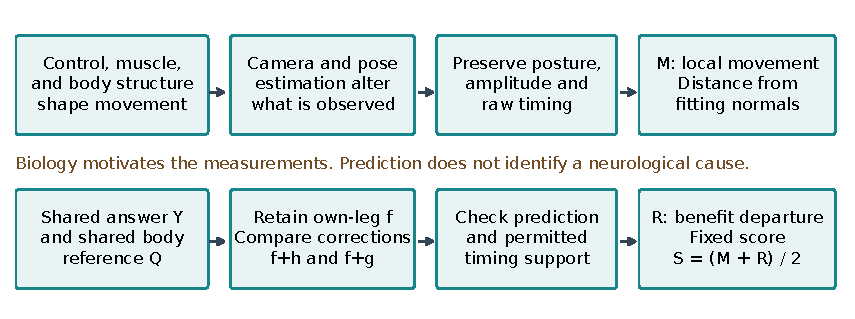
\includegraphics[width=\textwidth]{figures/method.pdf}
\caption{Biological reasoning motivates separate local movement and relational measurements. The three predictors share the same observable target and declared body reference. Prediction adequacy precedes interpretation; passing it does not guarantee added detection value.}
\label{fig:method}
\end{figure*}

\section{Related work and physiological motivation}

S-JEPA learns skeletal representations by predicting teacher features, while MAMP uses masked motion prediction \citep{abdelfattah2024sjepa, mao2023mamp}. Their motion-aware masking differs from our intentionally motion-independent reference. VideoMAE uses temporal tubes, and SLiM's semantic tubes already target anatomical reconstruction shortcuts \citep{tong2022videomae, do2026slim}. Our comparison controls token budgets, marginal probabilities and the downstream observation task; it does not claim those mask families are new. Stochastic positional queries are another intervention and remain separate from selecting hidden inputs \citep{bar2024stop}.

Normal-only gait methods already model posture, time and reconstruction. FSGait separates posture and temporal evidence; GenGait uses masked gait reconstruction and joint inconsistency \citep{duan2024fsgait, motta2026gengait}. SeeKer estimates conditional keypoint densities, and STG-NF learns pose likelihoods \citep{delic2025seeker, hirschorn2023stgnf}. Thus conditional surprise, normative reconstruction and multiple score channels are not sufficient novelty. Our empirical question concerns what an added-context predictor measures after local geometry, nominal residual width and observation support are controlled.

Post-stroke motor-module changes and weakness can alter sided movement and compensation \citep{clark2010modules, awad2020drive}. Parkinsonian movement size and arm coordination need not change together \citep{morris1994hypokinesia, sterling2015armswing}. Cerebral palsy combines varied motor-control and musculoskeletal constraints, while myopathic gait concerns muscle disease rather than a single brain disorder \citep{steele2015synergies, steele2012crouch, vandekerckhove2025dmd}. These findings motivate preserving amplitude, posture and timing as distinct observations. They do not establish that video predictability recovers neural synergies; mechanics and task constraints can also produce coordinated patterns \citep{kutch2012synergies}. A full movement world model would require control, mechanics, contact and observation components with multiple compatible explanations. We test only an observable completion component.

\section{Data and exploratory protocol}

\subsection{GAVD observation population}

We rebuild the inventory from the current condition CSVs, excluding the distribution folder. GAVD provides web recordings, sequence annotations and observed gait categories \citep{ranjan2025gavd, gavd2026catalog}. The inventory contains 1,874 sequences, 458,116 rows and 348 upload IDs. There are 332 decodable videos. Fixed pose-quality rules retain 311 sources; lower-limb readout support retains 304 sources, 1,381 sequences and 9,442 windows (Table \ref{tab:attrition}). A confirmed pixel-identical duplicate pair already fails pose quality, so the retained cohort has 304 known recording groups. Unknown repeated people remain unresolved.

\begin{table}[t]
\centering
\begin{tabular}{lrrr}
\toprule
Population & Sources & Normal & Windows \\
\midrule
Fresh annotations & 348 & 32 & -- \\
Pose-window quality & 311 & 28 & 9,474 \\
Lower-limb readout & 304 & 28 & 9,442 \\
Focal binary endpoint & 90 & 28 & 2,594 \\
Lab, selected & 188 & 138 & -- \\
Lab, eligible & 178 & 128 & 433 \\
\bottomrule
\end{tabular}
\caption{Observation attrition. GAVD units are upload IDs, not verified participants. Laboratory units are dataset participant IDs. Selection is part of the target population.}
\label{tab:attrition}
\end{table}

The focal primary contrasts normal with Parkinsons, stroke, cerebral palsy and myopathic memberships: 28, 10, 15, 10 and 27 sources, respectively. The broad secondary includes every non-normal folder with unchanged scores. One source has two abnormal memberships and counts once in binary endpoints. A frozen multi-membership exclusion leaves 89 sources for the separate supervised five-class task. Folder labels are not independently revalidated diagnoses; some broad categories describe circumstances rather than disease.

This is an exploratory redesign after an earlier completed context study. All 28 normal recordings had appeared in prior exploration. We froze the new population, endpoints, roles, masks and score before new fitting, but do not call the analysis confirmatory. Four outer folds each reserve seven test normals and five separate reference normals; the other 16 normals fit models. Abnormal sources enter only outer evaluation, except in separately labeled supervised comparators. Three source-grouped internal folds select the small residual grid. Reference normals never select architecture, signs, stopping or fusion. Overlapping windows, sequences and edits remain inside their source role. Fits share sources across folds and are not independent replications.

\subsection{Preserved measurements and restricted inputs}

The existing ingestion pipeline crops each annotated person using the frame-specific GAVD box, detects BlazePose landmarks, and restores full-frame coordinates \citep{bazarevsky2020blazepose}. It returns the first pose in the crop and is not a validated temporal identity tracker. We use raw coordinates, decoded-frame flags and confidence. Values below 0.5 remain missing. Resampling to 15 Hz interpolates only between adjacent valid source observations. Windows contain 32 samples with stride 16; all four samples must be valid for a token. Existing overall and half-window validity gates remain unchanged.

Only indices 11--16 and 23--32 enter masking: shoulders, elbows, wrists, hips, knees, ankles, heels and foot indices. Source readouts use the eight distal-leg joints, 25--32. The shared reference \(Q\) centers each frame on the pelvis and scales by valid first-half torso length. We do not rotate trunks upright, standardize each joint's excursion, or independently phase-align legs. Own-leg access is conditional on this shared body reference, which already contains body measurements. Projected angles and scaled image trajectories are not clinical three-dimensional angles, speed or ground clearance.

\section{Controlled prediction and masking}

Let \(O\) denote permitted visible own-leg tokens, \(C\) opposite-leg tokens, and \(Y\) the hidden four-frame XY target. Own-leg membership is hip, knee, ankle, heel and foot index. We apply masks and validity before constructing interpolation, temporal features or model inputs. Completion can use observations before and after the target; it is not future forecasting.

We fit a shared ridge baseline \(f\) on normal sources, freeze it, and compare

\begin{align}
\widehat Y_0 &= f(O;Q),\\
\widehat Y_o &= f(O;Q)+\alpha_o h(O;Q),\\
\widehat Y_b &= f(O;Q)+\alpha_b g(O,C;Q).
\end{align}

The local basis contains permitted interpolation estimates, support indicators, relative time and target identity. The own correction adds own-leg temporal moments; the bilateral correction adds opposite-leg features. The baseline has 77 features; each residual has 154 features, eight outputs and 1,240 coefficients including intercepts. Equal widths do not equalize numerical feature rank or inductive bias. Ranks count thresholded feature Gram-matrix eigenvalues, not ridge effective degrees of freedom. Recorded GAVD ranks include 111 for the own residual and 141 for the bilateral residual. A zero gate returns the saved baseline exactly, but does not guarantee held-out improvement or contain the separately fitted own correction.

Every fit uses 512 source-balanced window/mask presentations, with equal source/readout-joint loss weights. Internal validation chooses residual ridge penalty from \(\{0.1,1,10\}\) and multiplier from \(\{0,0.5,1\}\). A bilateral recipe passes only if it improves over both baseline and own correction in at least two of three internal folds and on their mean source risk. This operational rule is not a significance test. Internal selection averages source/joint-weighted requests; final scoring additionally merges repeated masks within physical window targets. We report this weighting difference. Separate generated dependency and conditional-independence fixtures, zero gates and hidden-input invariance test estimator behavior without pretending to simulate a disease.

\subsection{Equal-budget training, fixed evaluation}

A window has eight temporal patches and 16 joints, or 128 tokens. U uniformly hides 64 tokens. J uniformly selects one joint, hides its eight temporal tokens and uniformly fills 56 from the other 120. A chooses an anatomical group with probability equal to its width divided by 16. Four-joint groups are torso reference joints and either distal leg; two-joint groups are elbow and wrist on either side. Four-joint groups occupy two patches starting at 0, 2, 4 or 6; two-joint groups occupy four patches starting at 0 or 4. Starts are chosen uniformly from those listed. Each core has eight tokens. Uniformly filling 56 remaining tokens yields

\begin{equation}
P(\text{hidden})=\frac{1}{16}+\frac{15}{16}\frac{56}{120}=\frac12.
\end{equation}

All policies are motion-independent and share exact U-trained baseline weights. The coordinate target definition, nominal budget, unrelated RNG streams and source/window schedule are shared. Selected training targets and valid loss terms can differ. Matching marginals does not match higher-order dependence, difficulty or usable supervision. Masks are drawn before natural missingness, without favorable redrawing.

The primary U evaluation bank has 16 stored masks with seed 17 and preserves the historical own-joint support rule. The separate E\_leg bank enumerates two distal sides and four starts twice, fills to 64 with seed 117, and scores the forced core only. New training and E\_leg require a valid target and at least two permitted tokens at distinct times on each leg. Every source requires four distinct physical target patches per readout. Repeated masks cannot satisfy that requirement. Each bank uses the same five reserved reference identities and its own fitted reference parameters. All 304 sources retain support on both banks. A versus U on the unchanged U bank is the primary masking contrast; E\_leg cannot replace an unfavorable U result.

\section{Scores and evaluation}

The local channel \(M\) uses 16 descriptors from full observed movement. Each leg supplies knee-angle median and interquartile range, ankle X/Y interquartile ranges and velocity median absolute deviations. Trunk inclination median/IQR and two sided differences complete the vector. We average windows within sequences and sequences within sources before normal-only imputation, robust scaling and shrinkage covariance fitting. \(M\) is squared Mahalanobis distance divided by 16. These full-observation descriptors never enter a restricted completion branch.

For identical target coordinates, define benefit

\begin{equation}
b=\operatorname{MSE}(\widehat Y_o,Y)-\operatorname{MSE}(\widehat Y_b,Y).
\end{equation}

Masks average within targets, targets within windows, windows within sequences and sequences within sources, retaining joint identity. Four joints average equally on each side. Five reserved normal references supply bilateral means \(\mu_k\) and sample variances \(s_k^2\). We use \(v_k=0.5s_k^2+0.5\operatorname{mean}(s^2)+10^{-8}\) and \(R=\frac12\sum_k(b_k-\mu_k)^2/v_k\). The frozen score is \(S=(M+R)/2\). A failed internal gate would set \(R=0\) for every source in that fold; none failed. Neither benefit nor \(R\) is mutual information or a health ranking. Dimension normalization does not make M and R equally calibrated probabilities, and R omits bilateral covariance.

Comparators retain the same sources: a richer 36-feature motion distance; base-to-own sham benefit; equally constructed constituent-error fusions; timing/waveform descriptors; Isolation Forest; availability-and-viewpoint distance; and a separately supervised nuisance classifier. A bounded STG-NF adapter uses its authors' implementation with a 16-joint graph and fitting-normal median imputation. Native complete cases retain only five normal sources and cannot support the same roles. The adapter is not a faithful published reproduction. Separate five-class Random Forest and learned/random JEPA probes use source-separated labels. Fresh encoders pretrain only on fitting normals with EMA and VICReg \citep{bardes2022vicreg}; these small probes do not establish representation-learning limits.

We summarize AUROC by within-fold values weighted by fixed normal-by-abnormal pair counts. Average precision is reported per fold and as an equal-fold mean with prevalence. Pooled out-of-fold ranks are secondary because separate references need not align score scales. Paired 1,000-replicate bootstraps resample whole recording groups within fold and binary-label stratum, retain all method scores together and preserve original fold weights. Intervals condition on the fitted models, split and selected protocol; they omit fitting uncertainty, unknown repeated-person dependence and adaptive redesign. Multiple contrasts are exploratory and are not multiplicity-adjusted.

\subsection{Fixed-answer timing diagnostic}

For a valid 48-frame parent, frames 8:40 supply the target interval. Distal opposite-leg observations come from offsets \(-4\) or \(+4\) frames, without wraparound, padding or crossing annotations. Each donor vector is relative to its permitted donor hip, divided by the original scale, and attached to the permitted opposite hip at the original time. Original and shifted inputs share target, own leg, reference and pair-specific permitted support. A hidden donor coordinate cannot reappear after shifting. Sixteen stored uniform parent masks hide 96 of 192 tokens, with seed 217, before original/donor joint-and-hip visibility is intersected.

The estimand is shifted minus aligned squared error from the frozen bilateral predictor on identical targets. Zero-offset, own-branch invariance, noise, missing-observation and whole-body crop controls accompany it. Shifting also changes instantaneous geometry and finite-interval distributions, so even a successful effect would not isolate neural timing. Adequacy is rechecked on the exact paired original inputs rather than assumed from denser training inputs.

\section{Results}

\subsection{Completion, mask structure and detection}

All 12 outer-policy fits pass the internal normal gate. Direct interpolation is weaker than shared ridge in every aggregate of internal held-out GAVD normals. Figure \ref{fig:normal} shows outer-test normal errors. U-bank bilateral benefit remains uncertain for U and A; E\_leg provides more headroom. Thus an internal selection gate alone does not establish uniform-task generalization.

\begin{figure*}[t]
\centering
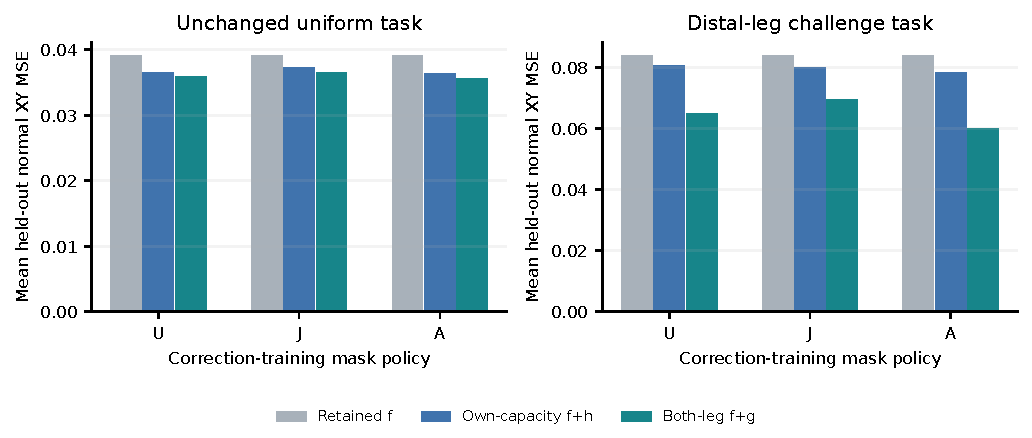
\includegraphics[width=\textwidth]{figures/normal_prediction.pdf}
\caption{Outer-test normal coordinate MSE, equally aggregated over sources. Every training policy retains the same U-trained baseline. The focused E\_leg bank changes the observation task and exposes more headroom; its errors must not be compared with U as an isolated training effect.}
\label{fig:normal}
\end{figure*}

\begin{table}[t]
\centering
\begin{tabular}{lrr}
\toprule
Score, U evaluation & Focal & Broad \\
\midrule
Local movement M & 0.694 & 0.707 \\
Relational departure R & 0.445 & 0.560 \\
Fixed S, U training & 0.576 & 0.631 \\
Richer motion, 36 features & 0.677 & 0.669 \\
M + own-capacity sham & 0.687 & 0.661 \\
M + constituent error & 0.684 & 0.685 \\
M + baseline error & 0.700 & 0.692 \\
Timing/waveform distance & 0.588 & 0.631 \\
Isolation Forest & 0.551 & 0.593 \\
STG-NF, adapted & 0.376 & 0.435 \\
Availability and viewpoint & 0.389 & 0.520 \\
Supervised nuisance & 0.461 & 0.506 \\
Fixed S, J training & 0.620 & 0.644 \\
Fixed S, A training & 0.631 & 0.672 \\
\bottomrule
\end{tabular}
\caption{Weighted within-fold AUROC. Focal and broad prevalence are 62/90 and 276/304. The fixed fusion has no demonstrated advantage. The adapted pose baseline and supervised nuisance row have distinct modeling assumptions.}
\label{tab:detection}
\end{table}

The primary S minus M contrast is -0.118, conditional 95\% interval {[}-0.217, -0.025{]}. The broad difference is -0.076, {[}-0.143, -0.009{]}. For the masking comparison, A minus U on the fixed U bank is 0.055, interval {[}-0.018, 0.127{]}, on the focal endpoint. This does not establish a better mask policy. The focal E\_leg S AUROCs for U, J and A are 0.668, 0.668, 0.684; they describe specialization to a different task. All arms and failures remain reported.

For U, focal equal-fold average precision is 0.763 for S and 0.864 for M; fold prevalence is 0.682, 0.696, 0.696, 0.682. High precision values must be read beside this high abnormal prevalence. Sham and constituent-error controls do not rescue the primary relational claim. The separate five-class equal-fold macro F1 values are 0.347 for Random Forest, 0.251 for learned JEPA and 0.309 for the random encoder. This modest classification comparison is not evidence of a clinical classifier or a JEPA advantage.

\subsection{Timing adequacy fails despite recording coverage}

The timing census retains 27 normal recordings, with 7, 7, 6 and 7 outer-test normals. It passes the operational coverage floor. However, all 24 outer fold/policy/offset combinations fail adequacy on their exact paired original inputs, as do all 72 corresponding internal combinations. Only about 1.75 editable distal tokens remain on average. U's negative offset has a positive raw effect of 0.000393, interval {[}0.000177, 0.000618{]}; the positive offset gives 0.000064, interval {[}-0.000232, 0.000368{]}. The negative-offset interval excludes zero, but compares two predictions from a model that is inadequate on the aligned paired inputs. It therefore does not establish a reliable coordination measurement (Figure \ref{fig:timing}). Software identity and visibility tests pass, but do not repair insufficient useful context.

\begin{figure*}[t]
\centering
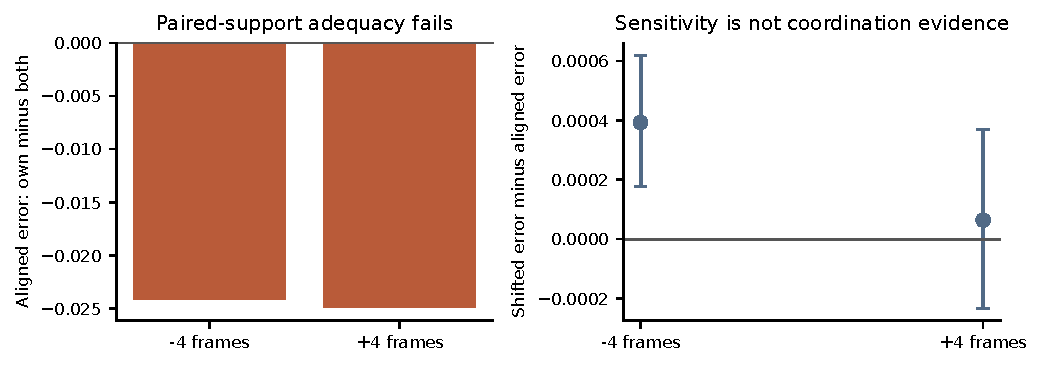
\includegraphics[width=\textwidth]{figures/timing_limits.pdf}
\caption{The U-trained predictor on 27 outer-test normal recordings separates a raw offset response from prediction adequacy on exactly matched inputs. All outer paired-support gates fail. A positive response alone is therefore insufficient for a timing interpretation. Error bars are conditional source-resampling intervals.}
\label{fig:timing}
\end{figure*}

\subsection{Independent participant replication}

We independently fit the same retained-prediction contrast to six simultaneous hip, knee and ankle flexion signals from a public laboratory dataset \citep{vancriekinge2023dataset}. One frozen walking trial per participant was selected before outcomes. All 188 selected trials parse; ten healthy trials fail unchanged observation support. The resulting 128 healthy and 50 stroke participants supply 433 windows. C3D angle declarations, degree units and common timestamps are verified. The first flexion component is not a global-axis rotation, and the signals are processed Plug-in Gait outputs with a shared body model.

The external representation uses 48 angle-patch tokens, half hidden, and the same gate logic. Each fold has 76 fitting healthy participants, 20 references and 32 healthy tests. Twelve angle median/IQR descriptors replace the image-specific M features. No limbs are independently cycle-aligned, no laboratory markers are relabeled as BlazePose joints, and no video weights are transferred.

All four internal gates pass. Bilateral prediction improves held-out healthy error over the own-capacity control by 4.78\% to 5.52\% across folds. A post-outcome audit on the frozen normal targets gives mean participant MSEs of 309.838 for direct interpolation, 206.262 for f, 201.038 for f+h and 190.584 for f+g, in squared degrees. The same ordering holds in every fold. Equal residual width still does not equalize rank: the 72-feature own and bilateral bases have ranks 44 and 62. The observed improvement applies to these fitted predictor families; it does not isolate opposite-leg information from every difference in effective flexibility.

Despite useful completion, M reaches 0.958 and S 0.892, difference -0.066, {[}-0.106, -0.031{]}. R alone reaches 0.694, so the negative finding concerns incremental value under this score construction, not absence of all abnormality information. A frozen same-sex, within-five-year matching rule retains 45 participant pairs; M reaches 0.955 and S 0.874, difference -0.081, {[}-0.156, -0.028{]}. Walking speed remains unmatched. Figure \ref{fig:delta} summarizes the consistent loss for the fixed fusion across measurement systems.

\begin{figure}[t]
\centering
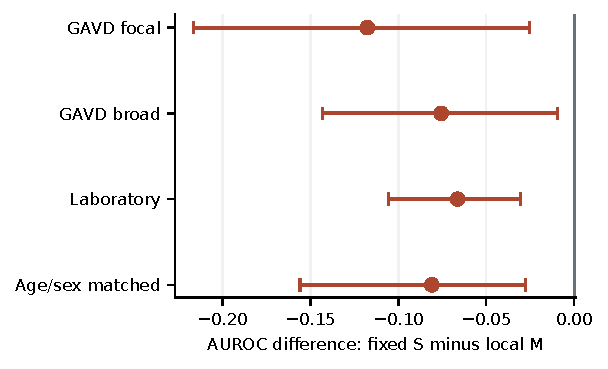
\includegraphics[width=\columnwidth]{figures/detection_difference.pdf}
\caption{S minus M AUROC with conditional 95\% intervals. GAVD intervals resample recording groups; external intervals resample participants, or matched pairs in the demographic sensitivity. These are not four independent studies.}
\label{fig:delta}
\end{figure}

\section{Observation failures and limitations}

We inspect prespecified high/low prediction-error examples in each focal label, with local videos, pose overlays and first/middle/last annotated frames. The ten cases show camera motion, assistance, split-screen footage, limb overlap and feet leaving the image. Figure \ref{fig:cases} illustrates measured skeleton traces without redistributing source photographs. Three sampled frames do not establish continuous identity correctness, and visible descriptions are not clinical relabeling.

\begin{figure}[t]
\centering
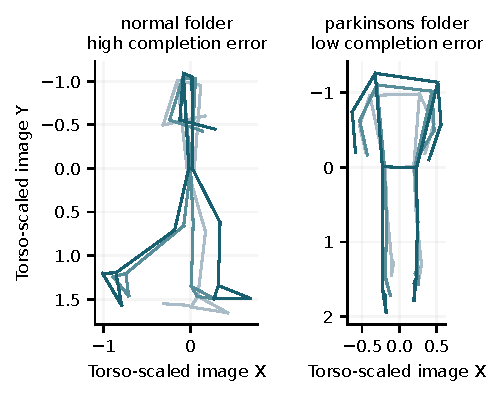
\includegraphics[width=\columnwidth]{figures/failure_cases.pdf}
\caption{Measured high-error normal and low-error Parkinsons-labeled examples. Sparse image traces are observation examples, not evidence that prediction error orders neurological severity. Source labels are retained without clinical reinterpretation.}
\label{fig:cases}
\end{figure}

A post-outcome boundary audit finds high-confidence distal points outside decoded images in frozen-window spans from 13/28 normal and 83/276 abnormal recordings. Pooled point fractions are approximately 0.43\% and 0.24\%; one requested frame fails decoding. Confidence therefore does not guarantee visible measurement, and the higher normal fraction cautions against attributing artifacts only to abnormal videos. No fits or exclusions change after this audit. Frame-aligned single-view strata lack enough normal support for a complete four-fold matched analysis; mixed views are not a matched viewpoint. Neither a global nuisance score nor the small camera review resolves these alternatives.

Five GAVD reference sources produce uncertain benefit scales. Saved leave-one-reference-out and variance-floor analyses expose that uncertainty. M and R also have different tails despite dimension normalization. In a post-outcome descriptive audit, external test-normal R 99th percentiles range from 6.30 to 33.94 across folds, versus 2.45 to 3.99 for M. External reference left/right benefit correlations range from 0.54 to 0.82, which the diagonal R distance does not model. These observations do not identify the cause of fusion loss. The negative result may reflect score calibration, reference estimation or representation choice as well as limited incremental movement information. We do not tune fusion after observing abnormal results. A new normal-only calibration study would require a separately frozen protocol and fresh evaluation.

The laboratory replication addresses participant separation and changes the observation system, but covers only healthy and stroke walking, excludes ten selected healthy trials and does not validate clinical deployment or video-weight transfer. GAVD remains an internal web-recording study with a small, previously explored normal sample. More abnormal windows do not replace independent normal participants. Conditional intervals omit training uncertainty, and limited ridge/JEPA budgets do not establish the best attainable model. The imputed STG-NF adapter is an informative bounded comparison, not a state-of-the-art benchmark.

\section{Conclusion}

Opposite-leg observations can improve normal movement completion while a fixed bilateral-benefit score worsens anomaly ranking. On incomplete video observations, even a positive timing response can coexist with failed prediction adequacy. A defensible relational detector must establish input access, useful prediction on its exact support, and incremental detection value separately. This study provides an executed test of those requirements and a narrow negative result across two measurement systems and partly different condition sets, without converting prediction behavior into a neurological diagnosis.
\bibliography{references}
\end{document}
